\documentclass{standalone}
\usepackage{tikz}
\usepackage{tkz-euclide}
\usepackage{ctex}
\setCJKmainfont{Noto Serif CJK SC}
\usepackage{mhchem,siunitx}
\begin{document}
\small
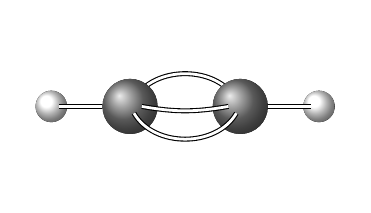
\begin{tikzpicture}[scale=1.0]
  \useasboundingbox(-2,-1)rectangle(2,1);
  \fill[ball color=white]([shift=(180:1.0)]-0.7,0)circle(0.2);
  \fill[ball color=white]([shift=(0:1.0)] 0.7,0)circle(0.2);
  \draw[double,double distance=1pt](-0.7,0)--++(180:0.9);
  \draw[double,double distance=1pt](0.7,0)--++(0:0.9);
  \draw[double,double distance=1pt]([shift=(60:0.1)]-0.7,0)to[out=60,in=120]([shift=(120:0.1)]0.7,0);
  \fill[ball color=gray](-0.7,0)circle(0.35);
  \fill[ball color=gray](0.7,0)circle(0.35);
  \draw[double,double distance=1pt]([shift=(-60:0.1)]-0.7,0)to[out=-60,in=-120]([shift=(-120:0.1)]0.7,0);
  \draw[double,double distance=1pt](-0.55,0)to[bend right=10](0.55,0);
\end{tikzpicture}
\end{document}